
\chapter{Introduction}
\label{chap:intro}
% o General: Start with very general description and focus step by step on your topic
% o keep in mind, that the introduction usually contains the most references
% o Introduction to main topic (e.g. Radiotherapy, MRI, ...) including historical review (1-2pages), Purpose of Radiotherapy ; Regardless of your actual topic, put it in context to conventional photon radiotherapy
% o Basic principles of Physics related to your topic
% o (e.g. Photo effect, Compton effect, Bethe-Bloch equation, ...)
% o Technological Background related to your topic
% o Give a general descriptions about the devices used in your thesis
% o (e.g. Linac, Afterloader, Synchrotron, Detectors...)
% o Overview of literature connected to your topic
% o Purpose of the thesis
% o based on the literature research, describe which information is missing, describe briefly what your thesis is about and what is the novelty of your work

\section{Photon - matter interactions}
\label{sec:photon}

As light passes through matter, its intensity decreases.
This phenomenon is due to photons interacting with electrons, nuclei, and their electric fields.
All processes either change the direction they travels in, alter it's energy, or result in the disappearance of single photons.
The probability of those interactions differ for each material (dependent on its density; proton number $Z$) and photon energy ($h\nu$). \\

If a photon's energy exceeds the binding energy of an orbital electron, the \textbf{photoelectric interaction} might occur.
Also known as 'photo effect', it describes a photon being completely absorbed by a tightly bound orbital electron which then is ejected from its atom.
The now free electron is called 'photo-electron'. Its kinetic Energy is the difference of the photons energy and the binding energy:
\begin{align}
E_{kin} &= h\nu - E_{binding}
\end{align} \\

Instead of being absorbed, photons might just 'bounce off' electrons or entire atoms, transferring momentum and in some cases a part of their energy to the electron.
\textbf{Rayleigh (coherent) scattering} happens when a photon interacts with a tightly bound orbital electron (transferring momentum to the entire atom).
This event can be seen as elastic, because only a negligible part of the photon's energy is transferred.

The \textbf{Compton effect (incoherent scattering)} involves a essentially free electron, such as an orbital electron with a relatively small binding energy compared to the photon's energy.
Due to the weak binding, momentum is transferred only to the electron.
This 'recoil electron' (or 'Compton electron') leaves its atom with a significant kinetic energy, which originated from the scattered photon.
Since the photon loses part of its energy, the event is considered inelastic. \\

When a photon with an energy above $1.02 \, MeV$ passes through the electric field of a nucleus, it might disappear to create an electron-positron pair.
This effect is called \textbf{pair production}.
The threshold of $1.02 \, MeV$ equals exactly the rest mass $E_m = 2m_ec^2$ for the two equally heavy particles.
The new particles travel in opposite directions with the same kinetic energy
\begin{align}
 E_{kin} = \frac{h\nu - 1.02 \, MeV}{2}
\end{align} \\

A photon with energy of the order of $2 \, MeV$ or higher can also interact directly with the nucleus.
Such a \textbf{Photonuclear reaction} is similar to the photo effect, in the sense that the photon is completely absorbed.
Its energy is transferred to the nucleus resulting in the emission of either a proton or neutron. \cite{Podgorsak, Maidment2014}\\

\subsubsection{Attenuation}
All those interactions result in a gradual decrease of light intensity as it travels through matter.
The combined effect is described by \textbf{Beer's law}:

\begin{align}
I(x) = I_0 e^{-\mu(h\nu,Z)x}
\end{align}

where $x$ is the thickness of a homogeneous material and $\mu$ its linear attenuation coefficient.
The different probabilities for the interactions to occur is implicitly considered by the attenuation coefficient $\mu(h\nu,Z)$ (see Figure \ref{fig:attenuation_water} and \ref{fig:attenuation_iron}).

For a photon being transmitted through matter with varying properties, the attenuation coefficient changes, too.
After travelling a distance d, the intensity can be expressed as:

\begin{align}
\label{eq:mu_int}
I(x) = I_0 e^{- \int_{0}^{d} \mu(x)dx}
\end{align}

Where $\mu(x)$ describes the attenuation at every distance $x$.

\begin{figure}[h!]
	\centering
	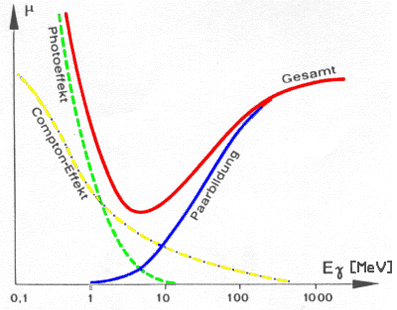
\includegraphics[width=0.5\linewidth]{/intro/attenuation_e}
	\caption{Photon attenuation schematic \\		\url{http://www.onmeda.de/strahlenmedizin/ionisierende_strahlung_reichweite-schwaechungsgesetz,-reichweite-von-photonenstrahlung-2413-6.html}}
	\label{fig:attenuation_water}
\end{figure}

\todo{better diagramm??}

\begin{figure}[h!]
	\centering
	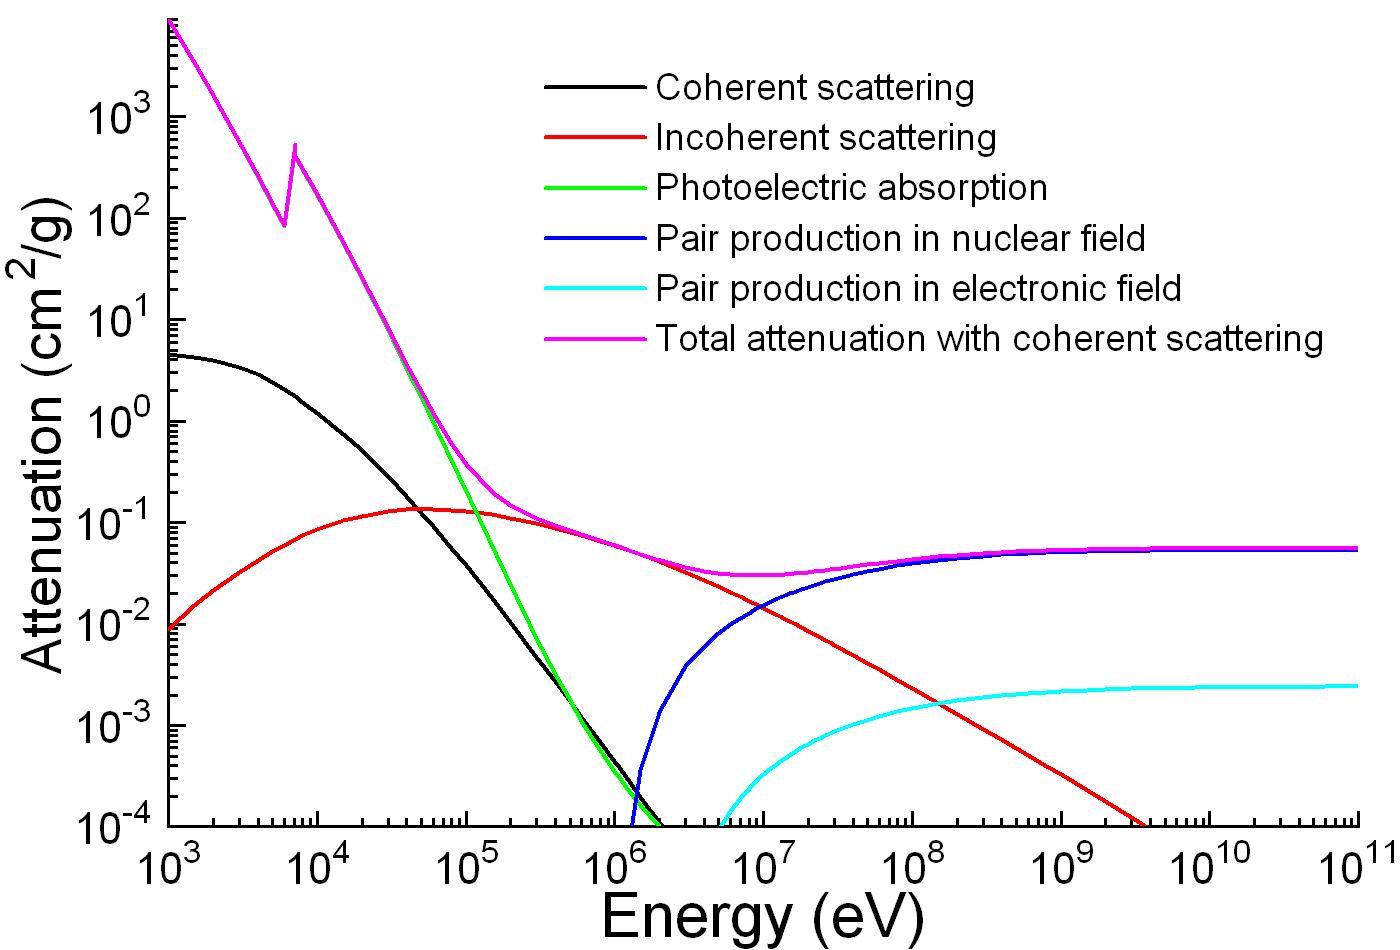
\includegraphics[width=0.7\linewidth]{../fig/intro/Ironattenuation}
	\caption{Photon attenuation for iron \\ \url{https://commons.wikimedia.org/wiki/File:Ironattenuation.PNG?uselang=en}}
	\label{fig:attenuation_iron}
\end{figure}


\section{Radiobiology}
\label{sec:cell}
\subsection{The human cell}
All living creatures consist of cells working together to form what is called tissue.
A collection of tissues which perform one or more functions is considered an organ. \\

Even though different types of cells serve different causes, all of them originated from the same totipotent zygote containing a original set of DNA.
A zygote is a stem cell, it has the ability to replicate indefinitely, passing on its DNA to the daughter cells.
At the same time it can change into any type of body cell. This feature is why it is called 'totipotent'.
As soon as the zygote has divided into a sufficient of identical cells, all of them differentiate into the various human tissues.
In favour of becoming more specialised cells, they lose their totipotency.
During the early stages of an embryo they are still capable of developing into a number of different cell types, but all within their own tissue type  either nerve, skin or blood \& muscle.
As those cells further specialise, they limit their potential even more.
In a fully grown human body there are still stem cells present, like bone marrow stem cells.
Other than the zygote, bone marrow can only give rise to blood cells, but not to e.g. nerve or skin cells.
A blood cell itself cannot replicate, it is considered a 'mature cell'.

The whole process follows the guidelines dictated by the DNA. Every cell inherited its own personal copy of the original set.
Inevitably mistakes happen during the replication, resulting in changes to the DNA called 'mutation'.
Most of these alterations are repaired or do not lead to changes in the cells behaviour.
As the human body ages the repair mechanism slows down and mutations accumulate.
At one point a cell is reprogrammed to act in a unpredictable way, giving up its duties and duplicating without restraint, forming tumours.
External factors are known influence cell behaviour and able to induce such 'malign' cells (carcinogenesis).
Cancer cells usually replicate more frequent than healthy cells, eventually leading to characteristic symptoms.

Different approaches have been developed to treat chancer, not all of which are suited to tackle every type of tumour.
If the tumour's location is unknown or metastases in many places have formed already, chemotherapy might be considered.
An easily accessible tumour could be removed in a surgery.
Non invasive therapies also include radiotherapy, destroying cancer cells using radiation.

Generally, early treatments have high chances of success, but tumours are often not noticed until they reached a certain stage. 
Reliable ways of diagnosing tumours are made possible by imaging techniques visualising the interior of the human body.  \cite{Baumann2017} \todo{Citation needed! Or should I take it out completely?}

\subsection{Effects of radiation}

As described in \ref{sec:photon}, light passing through matter transfer some of its energy to the medium.
Most interactions, such as the photo effect, incoherent (Compton) scattering, and pair production result in electrons being freed from their atoms.
If the electron has a sufficiently high kinetic Energy, it may free additional orbital electrons from surrounding atoms.
The remaining ions are positively charged, with a single unpaired valence electron.
This type of chemical is called 'radical' and considered extremely reactive.
They are likely to take part in chemical events which include the breakage of chemical bonds.
Such processes can either induce changes in DNA sequences and eventually produce biological damage.

A irradiated cell can be affected in various ways ranging from no effect to cell death.
The cell might survive containing a minor mutation.
A more fundamental mutation might lead to carcinogenesis.
Irradiated cells might send signals to their neighbours, inducing genetic damage known as 'bystander effects'.
Cells have been observed to react to radiation, becoming more resistant to future irradiation.

Changes to the DNA might not become apparent ever, others take years until they result in biological effects.
A well known consequence of ionizing radiation is leukaemia.
Damage to germ cells (sperm and eggs) might even result in genetic damages expressed in subsequent generations.

While imaging modalities utilising X-rays are designed to apply as little dose as possible to keep effects of irradiation low, radiotherapy makes use of the lethal effects targeting cancer cells. \cite{Podgorsak, Maidment2014}

\section{Imaging modalities}
\subsection{X-ray projection imaging}
A widely used imaging technique based on photon interactions is X-ray projection.
Its setup is made up by a light source, the object of interest, and a receptor.
Since the technique is about projection, a patient needs to be placed between an X-ray tube and the receptor (usually film-cassette or digital sensor).
In the first stage of the imaging process, X-ray photons emitted by the tube enter the body.
Next, while travelling through human tissue, they interact with its atoms in various ways (see \ref{sec:photon}).
These processes govern how much light is absorbed or scattered.
Finally, Photons which make it through the patient are recorded as they reach the receptor on the opposite side.
This results in a negative greyscale image, where brightness values correspond to the intensity reduction.
Low intensity (= high absorption) leads to bright spots on the image and vice-versa.
The whole process could also be described as 'the projection of attenuation shadows on to the receptor', since the light absorption directly depends on the attenuation coefficient. The attenuation, on the other hand, depend on the tissue's properties (e.g. proton number Z, density, etc).
Consequently, the attenuation shadows depict inner structures of the patient.

Soft tissue such as brain matter and muscles absorb only little light, casting a lighter shadow (dark areas on image) than bone which absorbs more photons (bright areas).
Anything other than bone differs only slightly in attenuation, owing to the relatively small difference in atomic numbers and density.
For this reason, X-ray projection imaging can be used to diagnose bone fractures, while at the same time it is not suited to clearly delineate soft tissue structures.
 
Other imaging modalities are better suited for the latter like medical ultrasound and Magnetic Resonance Imaging (MRI), to name a few. They are preferred for non invasive soft tissue examinations.
If those imaging modalities are no option, X-ray projection can still be of some use in combination with contrast agents.
Those substances fill e.g. the bloodstream with heavier atoms, which can be clearly seen against the dark background of surrounding soft-tissue.
In CT angiography, for instance, iodine is administered intravenously enhancing vessel to vessel-wall contrast.
In studies of the abdomen a diluted iodine solution or barium compounds swallowed by the patient leads improved visibility of the gastrointestinal tract.

For patients allergic to those chemicals, a number of alternative agents have been developed.
Unfortunately most introduce slight, sometimes serious side-effects.
There is ongoing research to find materials yielding enhanced contrast while at the same time minimising adverse reactions, a promising candidate being gold nanoparticles. \cite{Podgorsak, Maidment2014}


\subsection{Computer Tomography - CT}
Computer Tomography (CT) is a three-dimensional (3-D) imaging modality based on the measurement of X-ray attenuation.
The technique has evolved from 2-D X-ray scanning.
By mounting source and receptor on a rotary ring with a patient at the centre, projections from any angle can be obtained.
However, in contrast to 2-D projection methods, the receptor resembles an arc made up by 800 to 900 neighbouring detector elements.
A single 'image' taken by the receptor is therefore only in 1-D.
Yet, by repeating this process from a sufficient number of different angles and along the entire patient (z-axis) a 3-D model can be computed.
In contrast to 2-D methods, where the patients interior is projected/compressed onto a flat image, CT preserves the exact location information. This feature lead to a radical improvement in diagnostics.	 \\

Since its clinical introduction in 1971, CT has become a widely used 3-D imaging modality for a range of applications including radiation oncology. Especially in radiation therapy, knowledge of the exact geometry is crucial, which is why CT plays such an important role in treatment planning (see \ref{sec:planning}). \cite{Podgorsak, Maidment2014}

\subsubsection{3-D image reconstruction}
As a photon passes through the patient, it encounters different materials associated with characteristic linear attenuation coefficients.
It is practical to think of the scanned body as a collection of $N = N_X\cdot N_Y\cdot N_Z$ finite size cubes ($\Delta x$ cube length) called 'voxels' (analogous to pixels in a 2-D digital photograph).
The entire model can then be regarded as a 3-D matrix, with the attenuation coefficients $\mu_i$ for all voxels as its entries.
Figure \ref{fig:voxel_matrix} represents a ($4, 4, 1$) matrix.
It depicts the path an X-ray may follow passing through voxels with different values $\mu_i$.
This discretisation allows us to change equation \ref{eq:mu_int} to:

\begin{align}
\label{eq:mu_sum}
I(x) = I_0 e^{- \sum\limits_{i=1}^{N_X} \mu_i \Delta x}
\end{align}

The initial and final intensities can be read of the settings of the X-ray tube and the detected signal.
Based on those values, image reconstruction algorithms derive the three-dimensional linear attenuation coefficient matrix.
For convenience the computed numbers are converted to Houndsfield Units, which are displayed in the final image. \cite{Podgorsak, Maidment2014}

\begin{figure}[!htb]
	\centering
	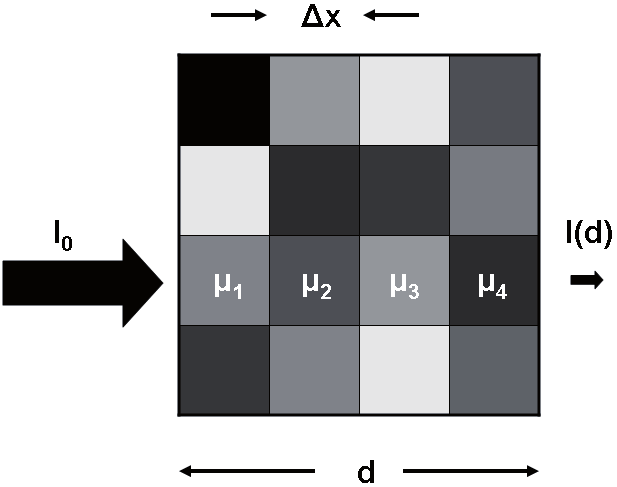
\includegraphics[width=0.5\linewidth]{intro/screenshot001.png}
	\caption{Simplified attenuation matrix (4,4,1)}
	\label{fig:voxel_matrix}
\end{figure}

\subsubsection{Houndsfield Units}

In a final CT scan voxel values are recorded in Houndsfield Units (HU), which relate to the attenuation of water at room temperature:

\begin{align}
HU_{material} = \frac{\mu_{material} - \mu_{water}}{\mu_{water}} \cdot 1000
\end{align}

Table \ref{tab:HU} lists types of human tissue and their values on the HU scale.
Generally HU values range from -1024 to +3071 (12 bit), but the upper limit can be extended to 15,359 (14 bit) if materials with even higher attenuation need to be visualised (e.g. implants).

\begin{table}[]
	\centering
	\caption{Average HU values for various types of human tissue}
	\label{tab:HU}
	\begin{tabular}{@{}ll@{}}
		\toprule
		Substance           & HU                     \\ \midrule
		Air                 & –1000                  \\
		Lung                & –750 (–950 to –600)    \\
		Fat                 & –90 (–100 to –80)      \\
		Water               & 0                      \\
		Muscle              & +25 (+10 to +40)       \\
		Brain, white matter & +25 (+20 to +30)       \\
		Kidneys             & +30 (+20 to +40)       \\
		Brain, grey matter  & +35 (+30 to +40)       \\
		Blood               & +55 (+50 to +60)       \\
		Liver               & +60 (+50 to +70)       \\
		Compact bone        & +1000 (+300 to +2500)  \\ \bottomrule
	\end{tabular}
\end{table}

Typically, CT scans are displayed on Computer monitors, which imposes the need to map the HU values to a 8-bit greyscale (256 steps of luminosity).
Since the number of possible values (dynamic range) on the HU scale is 16 times the shades of grey on a screen (12-8 = 4 bit difference; equivalent to a factor of $2^4$) the screen cannot convey all details at the same time.
A linear mapping would result in 16 neighbouring values being compressed to the same brightness.
This way, the brightest (bone) and darkest parts (soft tissue) of the image would be clearly distinguishable.
At the same time small differences (<16 HU) would appear as exactly the same intensity.
Generally however, the doctor's focus might lie either on soft tissue or bone material.
Bearing in mind that soft tissue values range only from 10 HU to 70 HU at most (see table \ref{tab:HU}), such a compression would make delineating organs using CT very unreliable.
Instead of showing detail from the lowest to the highest value, a window of values can be chosen.
Let's assume for example a range from -100 to 155 HU to be of interest.
This selected range can be mapped directly and uncompressed to a 8-bit greyscale.
Any values above 155 HU will be assigned the brightest value (white = 255), below -100 the darkest (black = 0).
While showing very good soft tissue contrast, all bones would be depicted with exactly the same brightness (255), even though they might have a varying HU values.
For bone structures a range from 300 to 2500 HU might show sufficient contrast.
Standard computer programs used to display CT images allow the user to change the window interactively to any value range. \cite{Podgorsak, Maidment2014}

\subsubsection{Image acquisition}
The time necessary to collect 1-D attenuation projections from sufficient angles is called 'acquisition time'.
In 2-D X-ray scanning only one picture is taken, while a 3-D CT model is made up of a photo sequence.
If the patient moves during the imaging process, the final model would show motion artefacts which might lead to wrong conclusions.
Consequently, CT scanners are designed to minimise acquisition time while ensuring sufficient image quality.
Very fast CT protocols result in smaller resolution, because less images are taken. \cite{Podgorsak, Maidment2014}

\subsubsection{Image quality} %282
CT offers excellent low contrast resolution, making structures that differ only slightly in signal from their surroundings visible to doctors.
This aspect of image quality is mainly limited by noise.
Noise is random patterns underlying the actual signal which always present to some extent.
It's prominence in the final image is described by the Signal to Noise Ratio (SNR).
If the SNR is too low, fine structures blend with the noise and cannot be distinguished. 
Strategies to achieve a high SNR include raising the initial photon flux (intensity) or employing contrast agents.
The intensity is governed by the tube current, which is limited by the heat capacity of the tube and health considerations regarding the patient.

Alternatively, the spatial resolution can be decreased, effectively combining neighbouring image slices.
While SNR for combined slices is increased, fine structures along the z-axis might be lost due to the reduced resolution. \cite{Podgorsak, Maidment2014}

\subsubsection{Health considerations}
CT scans describe the attenuation throughout a patient, which is directly related to how much energy is transferred from photons to matter.
Only because X-rays are absorbed by the human body, this imaging modality gives insight in the density distribution of a body's interior.
However, this transferred energy is capable of causing biological damage.
Fortunately the radiation dose administered during a single CT scan is almost negligible.
Nevertheless, cancer patients need to be imaged frequently during treatment planning.
Especially children receiving a great number of CTs typically suffer from induced cancer occurring up to 40 years later.
So while the benefit from using CT for diagnostics far outweighs the damage, there have been major efforts to reduce dose while maintaining reasonable image quality.
\cite{Murphy2007, Brenner2001, Sodickson2009, Smith2007, McCollough2009, Goldman2013}


\subsection{Magnetic Resonance Imaging - MRI}
Magnetic Resonance Imaging (MRI) is a 3-D imaging modality based on Nuclear Magnetic Resonance (NMR), a phenomenon discovered 1938 by physicist Isidor I. Rabi.
Atomic particles like protons have an inherent quantum mechanic feature called 'spin', which is associated with a magnetic moment $\mu$.
Without an external field a protons spin and magnetic moment is oriented in a random direction in space.
The sum of magnetic moments belonging to a great number of protons results in a net magnetisation.
Due to their random orientation, looked at from a great distance the net magnetisation will be zero.
On average for every proton's spin there is always another particle's spin oriented exactly the opposite way, cancelling its magnetic moment.

In the case of an applied external magnetic field, the spins will either align parallel or anti-parallel to the direction of this field, minimising their energy.
Protons aligned parallel have a slightly lower energy than those looking the other way.
In a collection of many spins, the number of parallel spins will therefore dominate, resulting in a net magnetisation other than zero.

By applying a radio frequency pulse the total external magnetic field changes and the magnetic moments start precessing around that new external field.
The additional pulse in usually exactly long enough to flip the spins by a $90^o$ angle.
They are now oriented in the transverse plane to the original external field.
Similar to a spinning top rotating not entirely upright, the magnetic moments will now precess around the direction of the external field.
Again they would like to minimise their energy by aligning with the external field, but in order to do so they need to give away the additional energy, transferring it to surrounding lattice.
Those spin-lattice interactions happen with different efficiency depending on the tissue.
The amount of time it takes for the spins to align is expressed in a material specific time constant $T_1$.
Shortly after applying the radio frequency pulse, regions of the body where magnetic moments align quickly (short $T_1$) have a stronger net magnetisation than those with energy being transferred slowly (long $T_2$).

At the same time the spins interact with each other, changing the local magnetic field.
The magnetic moments, which initially started out precessing in phase directly after the radio frequency pulse flipped them, will precess at slightly different frequencies, because of the small fluctuations in local magnetic field.
So after a while the net magnetisation in the transverse plane will vanish.
This process due to spin-spin interactions is described by the material specific time constant $T_2$

Eventually all spins will be again aligned either parallel or anti-parallel to the external field, just as they were before the rf-pulse. 


Measuring the net magnetisation throughout the body can therefore give information about tissue differences.


be measured with a pick-up coil surrounding the region of interest.

The nature of this effect leads to a great contrast between soft tissue. \cite{Currie2013}
Delineating tumours using MRI images is more accurate than using CT. \cite{Rasch1999, Debois1999a, Roach1996}

% mri needs coils
% mri can create differently weighted images (T1, T2, etc..)

\subsubsection{Image Quality}
Generally, diagnostics benefit from greater image quality.
However, at some point diagnostic accuracy stops increasing with field strength.
Nevertheless, high field scanners are key to developing new methods such as functional MRI (fMRI) of the brain \cite{Duyn2012} and observing ``metabolic reactions occurring in a human body in addition to producing very precise images of body structures'' \cite{Wada2010}.
At the same time astonishing improvements can be achieved at low fields.
A ``combination of field independent polarization [...] with frequency optimized MRI detection coils [...] results in low-field MRI sensitivity approaching and even rivaling that of high-field MRI.'' \cite{Coffey2013}

\subsubsection{Health considerations}

It's a glorified microwave!

\subsubsection{Open bore MRI scanners}

% advantages of low tesla, brachytherapy
The radiation oncology department of the Vienna General Hospital (AKH) is equipped with an 0.35T open-bore, c-arm MRI scanner.
The open design improves the well-being of patients experiencing anxiety in closed scanners.
Consequently, the number of incomplete MR examinations due to a claustrophobic events is low. \cite{Enders2011a, Bangard2007}
Besides, patients who wouldn't fit in closed designed scanners can be imaged.
Also, brachytherapy patients can be placed in the scanner with applicators attached.

This type of scanner is weaker than a conventional closed bore scanner (1-3 Tesla).
High field strengths would result in greater resolution, better Signal to Noise (SNR) ratio, and faster imaging time.
However, ``There are definite cost advantages (capital, operating, siting) to the use of lower field MRI.'' \cite{Rutt1996}
% capital, operating, siting????
Permanent magnets are sufficient to create the 0.35T field.
Therefore there is no need for constant cooling using liquid helium compared to superconducting magnets.
Consequently, maintenance and service costs are considerably lower.


\subsubsection{more stuff to be looked at}
One drawback of MRI, and especially open bore scanners, is the occuring distortion due to inhomogeneities in the magnetic field.
For most applications small position shifts and deformations are of minor importance.
In RTTP however, those effects can have a big impact.
Therefore MRI scanners usually come equipped with an internal distortion correction algorithm.
Those methods are developed by the company designing the scanners. Knowing the technical details enables them to drastically reduce the distortion.

Field of view (FOV) of the MRI scanner is smaller than the CT scanner's.

\section{External Beam Radiation Therapy}
\label{sec:planning}
External Beam Radiation Therapy (EBRT) utilizes ionizing radiation to damage cancer cells in order to stop them from multiplying.
This prevents the growth of tumours and eventually cures the patient. 
In conventional EBRT photons (x-rays) in the range of 4MeV to 20MeV are used to administer the necessary dose at the location of the tumour. Unfortunately, photons interact with all cells
they're passing through until they are fully stopped. They release their energy slowly while travelling through the patient and usually get completely absorbed after leaving the body.
Charged particles (e.g. protons, carbon ions) minimize the damage done to healthy tissue due to their distinctive behaviour in energy loss called ``Bragg Peak''.
They release most of their energy shortly before stopping. \cite{Nakamura2010} This effect can be used to spare tissue lying behind the tumour from radiation. \cite{Paganetti2005} % and before
A comparison between x-rays and protons is shown in figure \ref{fig:bragg}.

\begin{figure}[!h]
	\centering
	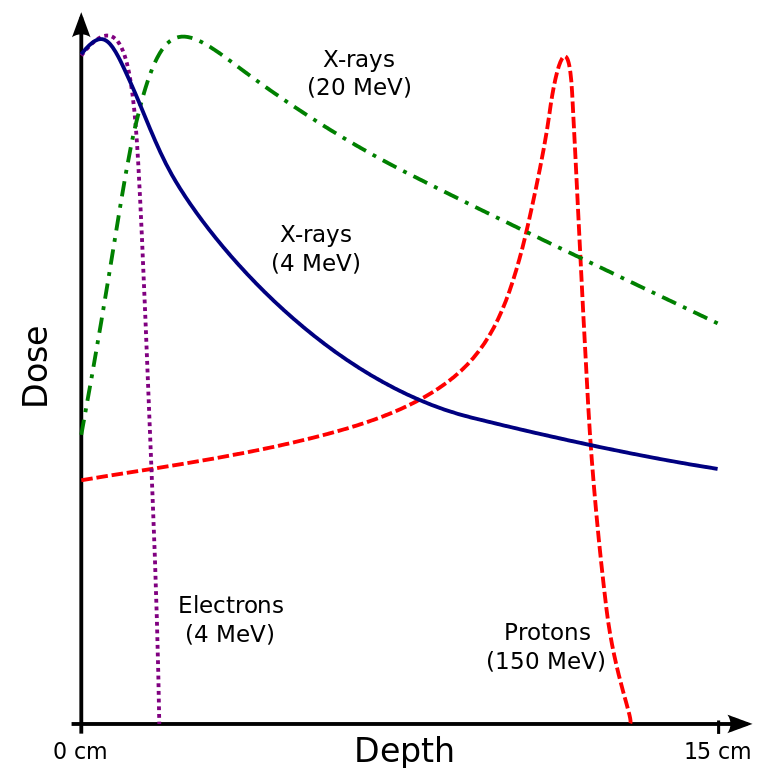
\includegraphics[width=0.6\textwidth]{Dose_Depth_Curves.png}
	\caption{energy release of ionizing radiation \\(By Cepheiden, via Wikimedia Common;\\ GFDL \url{http://www.gnu.org/copyleft/fdl.html})}
	\label{fig:bragg}
\end{figure}

While travelling through matter both types of radiation release energy mostly due to coulomb interactions with the outer shell electrons of atoms.
Knowing the electron density of of the targeted tissue area is therefore essential. In order to reach a specific penetration depth, the particles' initial energy has to be chosen accordingly.

\clearpage
\subsection{Role of CT}

Until recently radiotherapy treatment planning (RTTP) relied heavily on Computer Tomography (CT). There are two main reasons for this:

Firstly, CT uses low energy x-rays to create a 3D image of the patient. The luminosity value (brightness) assigned to each voxel (like pixel, but three-dimensional) corresponds to
the local radiodensity recorded in Hounsfield units ($HU$). Materials with a higher radiodensity (e.g. bones) absorb more x-ray photons than those with less (e.g. water, brain-mater).
Calculating the electron density using data obtained with CT is an easy task and used widely for RTTP. \cite{Constantinou2012, Schneider1996}
In order not to induce new cancer cells in healthy tissue during EBRT, the radiation beams are carefully targeted using the measured radiodensity. 
This way the absorbed dose accumulates in the cancer regions, while the nearby healthy tissue receives less radiation.

Secondly, CT images generate 3D images with little distortion. Exact geometries are needed for correct RTTP. %more details

\vspace{4cm}
\textit{Image of RTTP}
\vspace{2cm}

\subsection{Role of MRI}
There are some difficulties arising from combining CT and MRI for EBRT:
In order to profit from separately acquired data, the resulting images must be aligned either manually or automatically. This is a hard task since non-rigid objects (organs) change their shape and location between measurements. This leads to inaccuracies.
Therefore MRI-only radiation therapy protocols are being developed:
MRI data is used to create a Pseudo-CT, which contains information about electron density. Comparisons to using CT and MRI have shown acceptable deviations for X-ray therapy.
In charged particle therapy the resulting dose gain in healthy tissue and dose loss in cancer regions due to inaccurately assigned electron density values is bigger.
However, current development is promising. \cite{Rank2013, Stanescu2006, Nyholm2015, Greer2015, Chen2004}


Today RTTP often combines CT images with data acquired using Magnetic Resonance Imaging (MRI).
MRI scans also record luminosity values, but they do not correspond to $HU$ (radiodensity measured by CT).
The signal intensity depends on many factors and even varies between MRI scanners.



\section{Aim of this work}
The used open bore MRI scanner is not intended to be used for RTTP. The on board correction algorithm might not be good enough for effetive EBRT.
The goal of this work is to commence the development of a quality assurance tool to asses the spatial distortion (after applying the internal correction).
This is achieved by comparing MRI images to CT images used as a gold standard.
An alerady existing custom designed phantom is provided by the AKH Vienna for this purpose.
However, the liquid to fill the rods with has not been chosen yet.
Therefore, this paper focuses mainly on the acquired data and which liquids to use the phantom with, not its entire design.
However, possible fillings have to be produced and tested.
Similar approaches are being used for distortion correction by other facilities. \cite{Price2015, Petersch2004, Torfeh2015, Wang2004, Wang2004b, Mizowaki2000}


%to me \footnote{Auszug aus \citetitle{BohemRhap}~\cite{BohemRhap} von \citeauthor{Queen}~\cite{Queen} }\\
%\section{Farrokh Bulsara aka. Freddie Mercury}
%Farrokh Bulsara war ein Ausnahmetalent schuf zusammen mit der Band Queen einige der größten Hits aller Zeiten. Noch heute ist er ein wichtiges Thema in unterschiedlichsten Medien, wie in Abb. \ref{fig:freddiehg} zu sehen ist. %
%Weitere Zitate sind in Anhang \ref{appendix:zitate} zu finden.


\newpage